\section{Cinemática inversa do robô diferencial}

A cinemática direta do robô diferencial expressa como a velocidade linear ($v$) e a velocidade angular ($\omega$) do robô se relacionam com a velocidades das suas rodas, $\varphi_l$ e $\varphi_r$, que possuem raio $r$ e estão à uma distância $l$ do CG do robô. Tais relações são definidas em \eqref{eq:v} e \eqref{eq:w}, sendo compactadas de forma matricial em \eqref{eq:cinematicadireta}.

\begin{equation}\label{eq:v}
	v = \frac{r\varphi_r}{2} + \frac{r\varphi_l}{2}
\end{equation}

\begin{equation}\label{eq:w}
	\omega = \frac{r\varphi_r}{2l} - \frac{r\varphi_l}{2l}
\end{equation}

\begin{equation}\label{eq:cinematicadireta}
	\begin{bmatrix}
		v \\ \omega
	\end{bmatrix} = \begin{bmatrix}
	\frac{r}{2} & \frac{r}{2} \\
	\frac{r}{2l} & -\frac{r}{2l} 
	\end{bmatrix} \begin{bmatrix}
	\varphi_r \\ \varphi_l
	\end{bmatrix}
\end{equation}


Para que dada uma velocidade linear e angular desejas, o robô seja capaz de seguí-la, precisa-se saber qual a velocidade de cada roda deve desenvolver. Para isso, é utilizada a cinemática inversa, obtida ao isolar o vetor de velocidade das rodas em \eqref{eq:cinematicadireta}. Realizando tal procedimento, de acordo com \eqref{eq:cinematicainversa}, é obtida a relação da velocidade linear e angular que levam à velocidade das rodas do robô.


\begin{equation}\label{eq:cinematicainversa}
\begin{bmatrix}
	\varphi_r \\ \varphi_l
\end{bmatrix} = \begin{bmatrix}
	\frac{r}{2} & \frac{r}{2} \\
	\frac{r}{2l} & -\frac{r}{2l} 
\end{bmatrix} ^{-1} \begin{bmatrix}
v \\ \omega
\end{bmatrix} = \frac{\text{adj}\left(\begin{bmatrix}
\frac{r}{2} & \frac{r}{2} \\
\frac{r}{2l} & -\frac{r}{2l} 
\end{bmatrix}\right)}{\det{\left(\begin{bmatrix}
\frac{r}{2} & \frac{r}{2} \\
\frac{r}{2l} & -\frac{r}{2l} 
\end{bmatrix}\right)}}\begin{bmatrix}
v \\ \omega
\end{bmatrix} = \begin{bmatrix}
\frac{1}{r} & \frac{l}{r} \\
\frac{1}{r} & -\frac{l}{r} 
\end{bmatrix} \begin{bmatrix}
v \\ \omega \end{bmatrix}
\end{equation}

Foi realizada a validação por meio de simulação do modelo, obtendo a \autoref{fig:testcircledrive}, que demonstra que o modelo conseguiu desempenhar a trajetória desejada.

\begin{figure}[H]
	\centering
	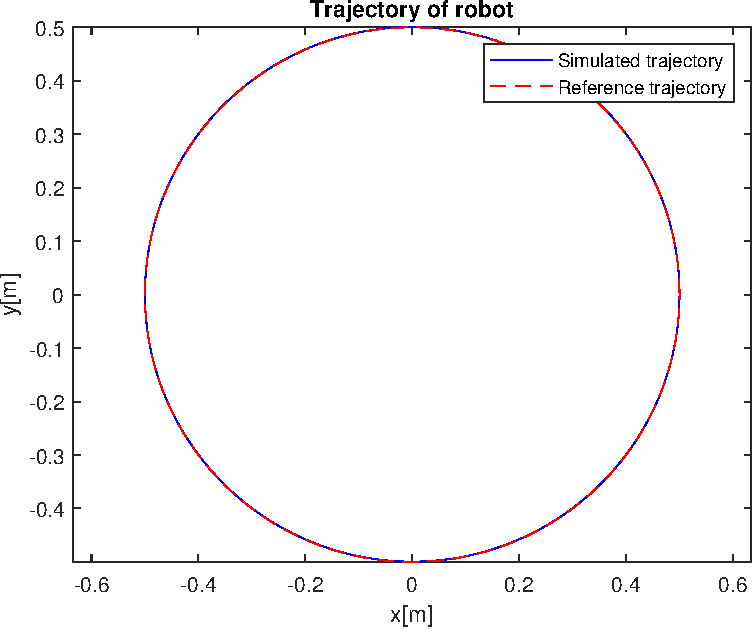
\includegraphics[width=0.5\linewidth]{img/testCircleDrive}
	\caption{Validação da cinemática inversa do robô.}
	\label{fig:testcircledrive}
\end{figure}




\section{Teleoperação do robô diferencial}

O algoritmo de teleoperação foi implementado de acordo com  o Algoritmo~\autoref{alg:teleop}.
\begin{algorithm}
	\caption{Algoritmo de teleoperação.}\label{alg:teleop}
	\begin{algorithmic}[1]
		\State $v \gets 0$;
		\State $\omega \gets 0$;
		\State $K \gets  \ $\Call{ReadKeyboardKey};
		\While{$K \ne \texttt{q}$}
			\Switch{$K$}
				\Case{\texttt w}:
				\State $v \gets v+0.1$;
				\EndCase
				\Case{\texttt s}:
				 \State $v \gets v-0.1$;
				\EndCase
				\Case{\texttt a}:
				\State $\omega \gets \omega+0.1$;
				\EndCase
				\Case{\texttt d}:
				\State $\omega \gets \omega-0.1$;
				\EndCase
				\Case{\texttt{SPACE}}:
				\State $v \gets 0$;
				\State $\omega \gets 0$;
				\EndCase
			\EndSwitch
			
			\State $[\varphi_l, \varphi_r] \gets $ \Call{calculateWheelSpeeds}{v, w, parameters};
			\State  \Call{setWheelSpeeds}{$\varphi_l$, $\varphi_l$}
			\State $K \gets  \ $\Call{ReadKeyboardKey};
			
		\EndWhile
	\end{algorithmic}
\end{algorithm}




\section{Controle em malha fechada}


Aplicado o controle em malha fechada, dado por \eqref{eq:controle}, obtêm-se o posicionamento do robô nas posições desejadas, como mostrado nas Figuras~\ref{fig:4-1},~\ref{fig:4-2}~e~\ref{fig:4-3}.

\begin{equation}\label{eq:controle}
	\begin{split}
		\rho &= \sqrt{(x_g-x)^2 + (y_g-y)^2} \\
		\alpha& = \mod \left[\text{atan2}\left(y_g-y,x_g-x\right) - \theta + \pi, \ 2\pi \right] -\pi \\
		v &= k_\rho\rho \\
		\omega &= k_\alpha\alpha
	\end{split}
\end{equation}

Sendo $k_\rho = 0,5$ e $k_\alpha = 1.5$, respeitando as condições para estabilidade do sistema.


\begin{figure}[H]
	\centering
	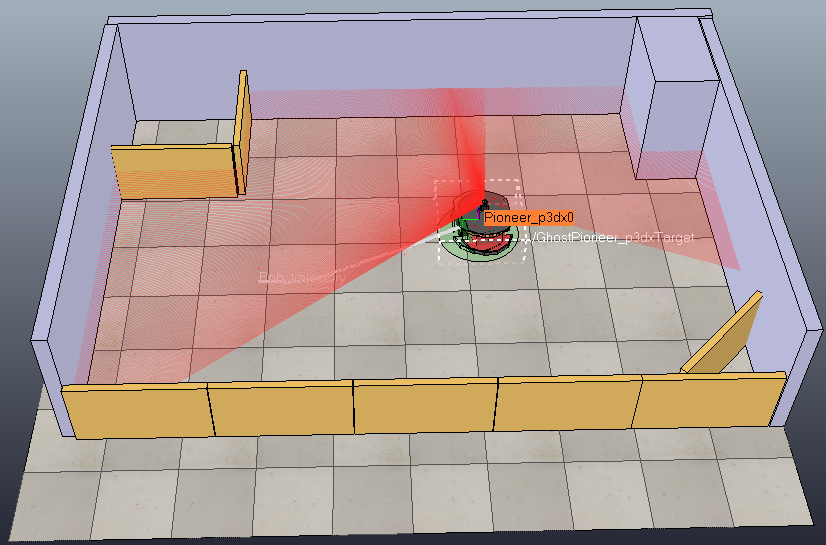
\includegraphics[width=0.6\linewidth]{img/4-1}
	\caption{Trajetória do robô para a posição $(1,6; 0,6)$ orientado à 90°.}
	\label{fig:4-1}
\end{figure}



\begin{figure}[H]
	\centering
	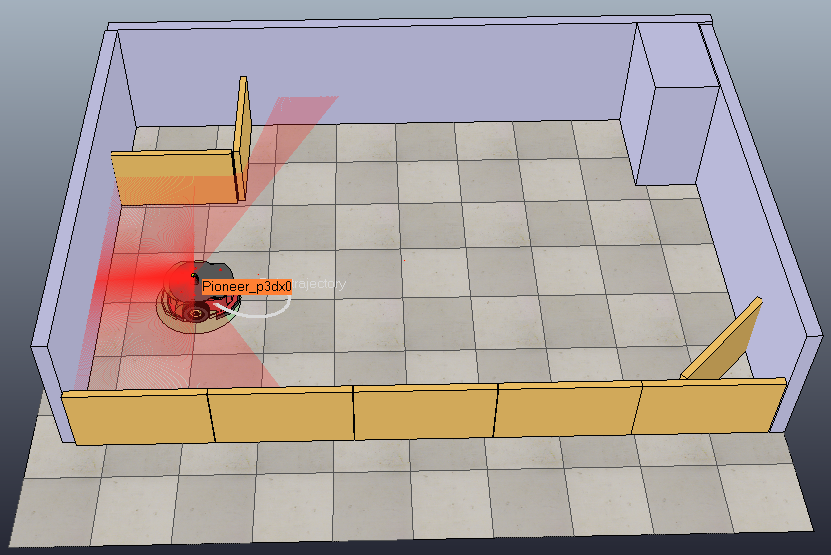
\includegraphics[width=0.6\linewidth]{img/4-2}
	\caption{Trajetória do robô para a posição $(-0,5; 0)$ orientado à 180°.}
	\label{fig:4-2}
\end{figure}


\begin{figure}[H]
	\centering
	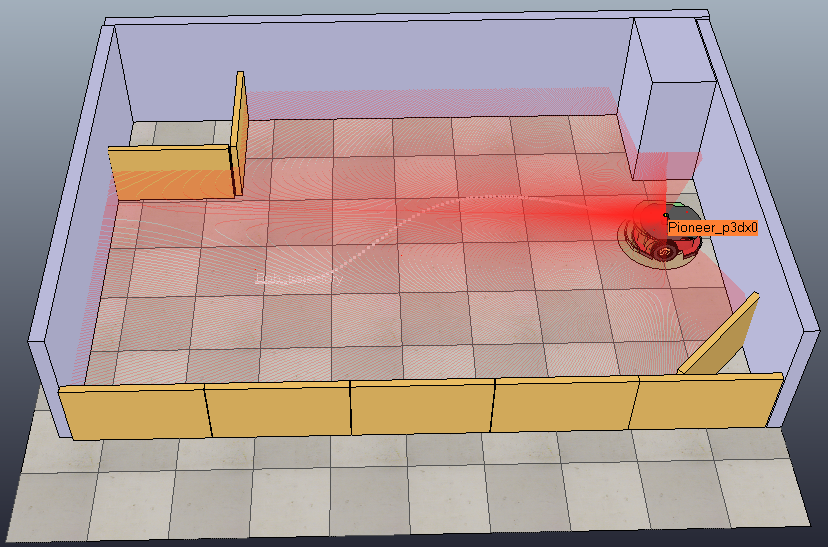
\includegraphics[width=0.6\linewidth]{img/4-3}
	\caption{Trajetória do robô para a posição $(3; 0,5)$ orientado à 180°.}
	\label{fig:4-3}
\end{figure}




\section{Controle melhorado}

A implantação de um controle melhorado, que possibilite o robô se mover para trás e conduzir em velocidade linear constante foi feita em duas partes: (i) Verificando se o robô deve seguir para frente ou para trás em direção ao destino; (ii) Obtendo a velocidade linear e angular para que o robô navegue em velocidade constante.

O Algoritmo~\ref{alg:direcao} verifica se o alvo se encontra à frente ou à trás do robô, por meio do ângulo de erro $\alpha$ entre a orientação do robô e a o ângulo do ponto de destino no sistema inercial. Com isso, caso $|\alpha| \le \pi/2 $, o mesmo deve se guiar para a frente, enquanto se $\alpha > \pi/2$, o mesmo deve se mover para trás. Para o segundo caso, a velocidade linear deve receber um sinal negativo, e o ângulo $\alpha$ ser acrecido de $\pi$, uma vez que o referencial de direção do robô passa à ser $-x$.

\begin{algorithm}
	\caption{Algoritmo de direção.}\label{alg:direcao}
	\begin{algorithmic}[1]
		\State $s_v \gets 1$;
		\If{backwardAllowed}
			\If{$|\alpha| > \pi/2$}
				\State $s_v \gets -1$;
				\State $\alpha \gets $ \Call{normalizeAngle}{$\alpha + \pi$};
			\EndIf
		\EndIf
		\end{algorithmic}
\end{algorithm}

\begin{algorithm}
\caption{Algoritmo de velocidade.}\label{alg:velocidade}
\begin{algorithmic}[1]
	\State $s_v \gets 1$;
	\If{useConstantSpeed}
	\If{$\rho > $ dist\_threshold $\cdot 2$}
	\State $\omega \gets \omega\cdot ($constantSpeed$/v)$;
	\State $v \gets $ constantSpeed $\cdot s_v$;
	\Else
	\State $\omega \gets \omega_i$;
	\State $v \gets v_i \cdot s_v$;
	\EndIf
	\EndIf
\end{algorithmic}
\end{algorithm}

A constante $\text{constantSpeed}/v$ calcula o quanto a velocidade linear do robô dada pelo controle foi alterada pelo uso da velocidade constante, fazendo a mesma compensação na velocidade angular, com intuito de manter a razão $v/\omega$ constante. Onde $v_i$ e $\omega_i$ são as velocidades lineares e angulares calculadas de acordo com o controle de~\eqref{eq:controle}. Foi necessário para um controle mais suave desativar a velocidade constante quando o robô está bem próximo do alvo, evitando a ocorrência de grandes velocidades angulares que geram \textit{overshoot}.

Como resultado, observou-se uma trajetória mais suave até o alvo, mas porém, com um tempo de missão maior, como mostrado nas Figuras~\ref{fig:5-1},~\ref{fig:5-2}~e~\ref{fig:5-3}.

\begin{figure}[H]
	\centering
	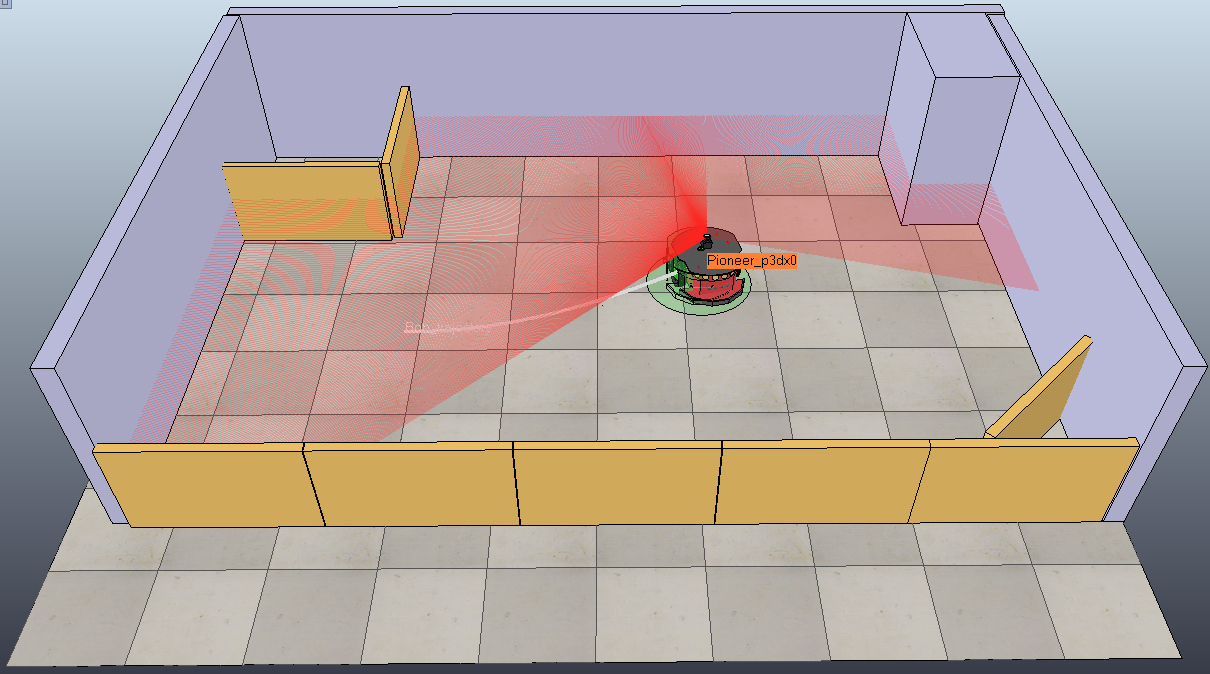
\includegraphics[width=0.6\linewidth]{img/5-1}
	\caption{Trajetória do robô para a posição $(1,6; 0,6)$ orientado à 90°.}
	\label{fig:5-1}
\end{figure}



\begin{figure}[H]
	\centering
	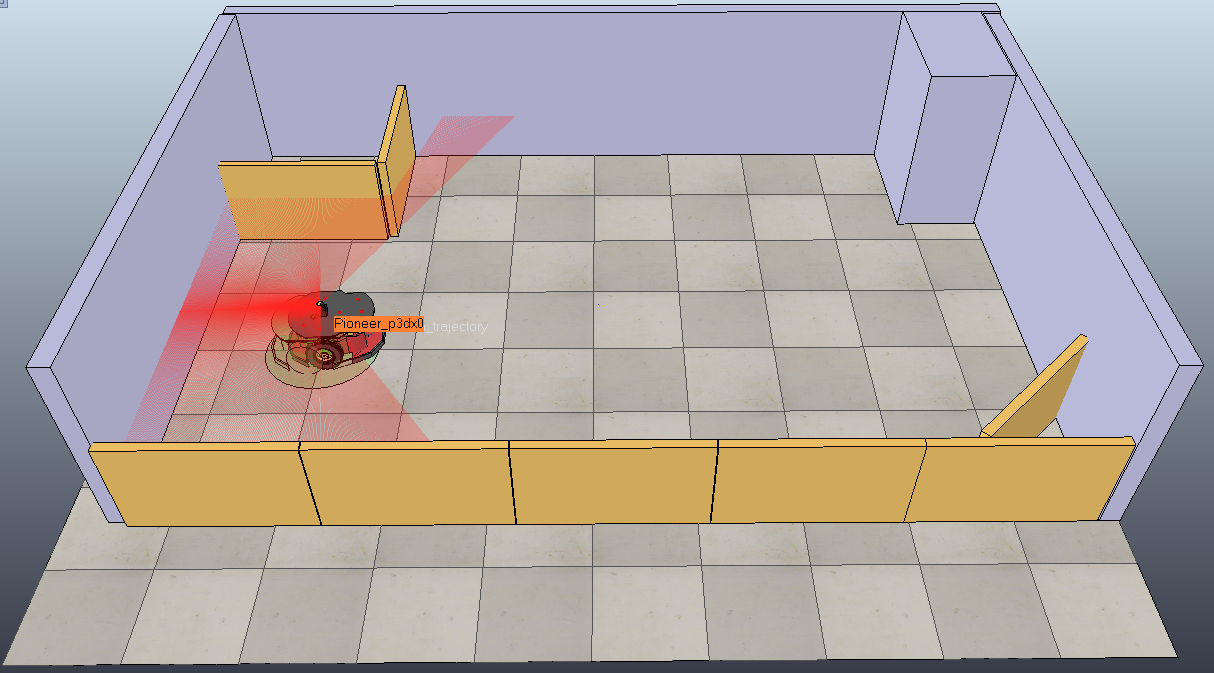
\includegraphics[width=0.6\linewidth]{img/5-2}
	\caption{Trajetória do robô para a posição $(-0,5; 0)$ orientado à 180°.}
	\label{fig:5-2}
\end{figure}


\begin{figure}[H]
	\centering
	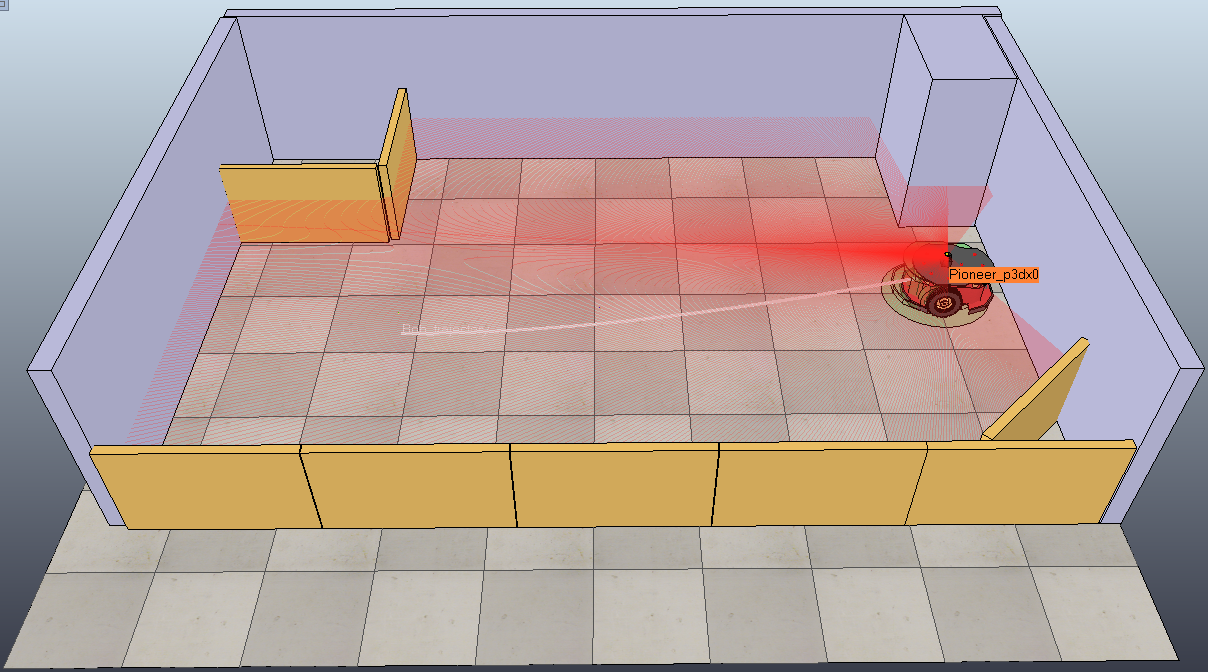
\includegraphics[width=0.6\linewidth]{img/5-3}
	\caption{Trajetória do robô para a posição $(3; 0,5)$ orientado à 180°.}
	\label{fig:5-3}
\end{figure}